\begin{figure}[tp]
\begin{centering}
    {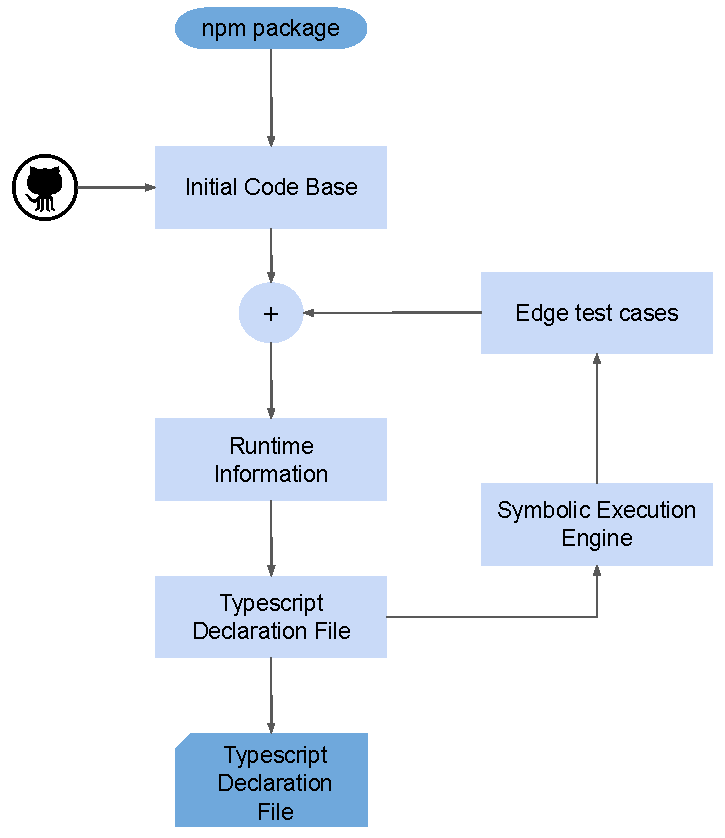
\includegraphics[width=0.9\textwidth]{figures/approach/typescript-declaration-files-generation-method/typescript_declaration_files_generation_method_block_diagram.pdf}}
    \caption[TypeScript Declaration Files Generation Method]{\textbf{TypeScript Declaration Files Generation Method} - Initial code base is retrieved from the npm package's repository. A valid TypeScript Declaration File is generated using run-time information. A Symbolic Execution Engine creates test cases based on the generated Declaration File and via a feedback loop enriches the code base until the stopping criteria is reached. The final TypeScript Declaration File gets returned. Feedback loop through the Symbolic Execution Engine was not implemented. It can be added in a future to the existing architecture, without modifying the working blocks.}
    \label{fig:tsd_generation_method_block_diagram}
\end{centering}
\end{figure}
